\chapter{Efficiënte zoekbomen}
\section{Inleiding}
\begin{itemize}
    \item Uitvoeringstijd van operaties (zoeken, toevoegen, verwijderen) op een binaire zoekboom met hoogte $h$ is $O(h)$ ($h = \lg n$).
    \item De hoogte $h$ is afhankelijk van de toevoegvolgorde van de $n$ elementen:
    \begin{itemize}
        \item In het slechtste geval bekomt men een gelinkte lijst, zodat $h = O(n)$.
        %\item Als elke toevoegvolgorde even waarschijnlijk is, dan is de verwachtingswaarde voor de hoogte $h = O(\lg n)$.
        %\begin{itemize}
        %    \alert Geen realistische veronderstelling.
        %\end{itemize}
    \end{itemize}
    \item \textbf{Drie manieren} om de efficiëntie van zoekbomen te verbeteren:
    \begin{enumerate}
        \item \textbf{Elke operatie steeds efficiënt maken.}
        \begin{itemize}
            %\item AVL-bomen. %(figuur \ref{fig:AVL-tree}).
            %\begin{figure}[ht]
            %    \centering
            %    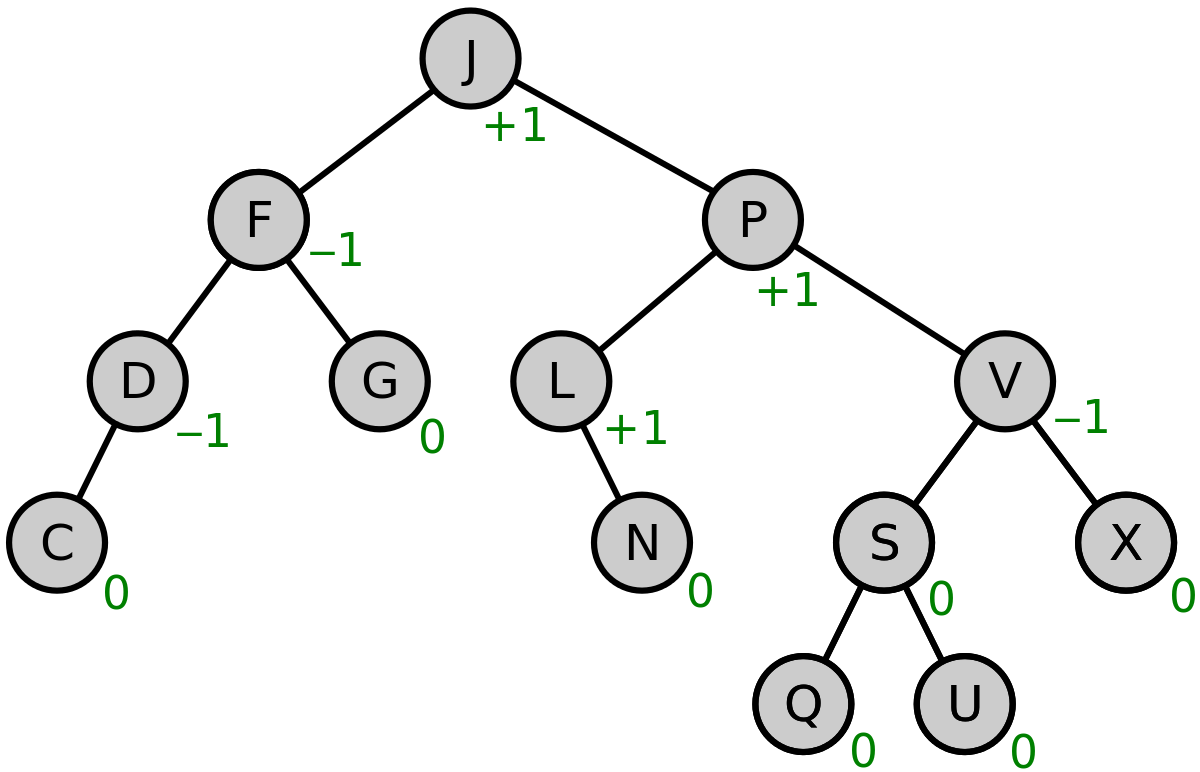
\includegraphics[width=0.5\textwidth]{AVL-tree}
            %    \caption{Een AVL-boom. De groene cijfers stellen de hoogteverschillen voor van de twee deelbomen voor elke knoop.}
            %    \label{fig:AVL-tree}
            %\end{figure}
            %\begin{itemize}
            %    \item Hoogteverschil van de tweede deelbomen van elke knoop wordt gedefinieerd als:
            %    $$\Delta h <= 1$$
            %    \item $\Delta h$ wordt opgeslagen in de knoop zelf.
            %\end{itemize}
            %\item 2-3-bomen (figuur \ref{fig:2-3-tree}).
            %\begin{figure}[ht]
            %    \centering
            %    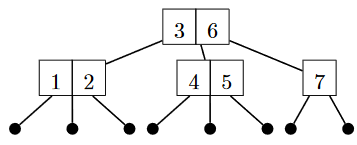
\includegraphics[width=0.5\textwidth]{2-3-tree}
            %    \caption{Een 2-3-boom.}
            %    \label{fig:2-3-tree}
            %\end{figure}
            %\begin{itemize}
            %    \item Elke knoop heeft 2 of 3 kinderen en dus 1 of 2 sleutels.
            %    \item Elk blad heeft dezelfde diepte.
            %    \item Bij toevoegen of verwijderen wordt het ideale evenwicht behouden door het aantal kinderen van de knopen te manipuleren.
            %\end{itemize}
            %\item 2-3-4-bomen.
            %\begin{itemize}
            %    \item Analoog aan een 2-3-boom, maar elke knoop heeft 2, 3 of 4 kinderen.
            %    \alert Per knoop moet er plaats voorzien zijn voor 3 sleutels, wat onnodig veel geheugen vraagt.
            %\end{itemize}
            \item Rood-zwarte bomen (sectie \ref{sec:rood-zwarte bomen}).
        \end{itemize}

        \item \textbf{Elke reeks operaties steeds efficiënt maken.}
        \begin{itemize}
            \item Splaybomen (sectie \ref{sec:splaybomen}).
        \end{itemize}

        \item \textbf{De gemiddelde efficiëntie onafhankelijk maken van de operatievolgorde.}
        \begin{itemize}
            \item Gerandomiseerde zoekbomen (sectie \ref{sec:gerandomiseerde-zoekbomen}).

        \end{itemize}
    \end{enumerate}
\end{itemize}

\section{Rood-zwarte bomen}
\label{sec:rood-zwarte bomen}
%\begin{figure}[ht]
%    \centering
%    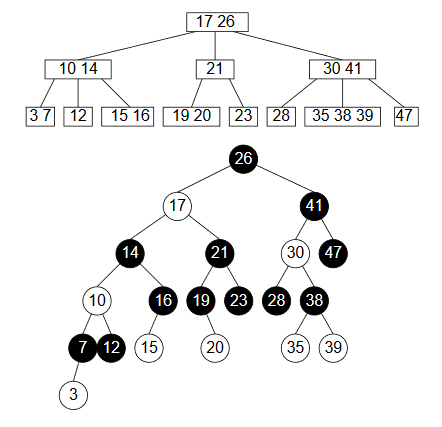
\includegraphics[width=0.5\textwidth]{2-3-4-RB-tree}
%    \caption{Een 2-3-4-boom en equivalent rood-zwarte boom (wit stelt hier rood voor).}
%    \label{fig:red-black-tree}
%\end{figure}
%\begin{itemize}
%    \item Simuleert een 2-3-4-boom (fig \ref{fig:red-black-tree}).
%    \begin{itemize}
%        \item Een knoop in een 2-3-4 boom worden 1, 2 of 3 knopen in een rood-zwarte boom.
%        \item Een 2-knoop wordt een zwarte knoop.
%        \item Een 3-knoop wordt een zwarte knoop met een rood kind.
%        \item Een 4-knoop wordt een zwarte knoop met twee rode kinderen.
%    \end{itemize}
%    \item Een rood-zwarte boom is gemakkelijker te definieren als er afgestapt wordt van het 2-3-4-boom concept.
%\end{itemize}
\subsection{Definitie en eigenschappen}


\begin{itemize}
    \item \textbf{Definitie:}
    \begin{itemize}
        \item Een binaire zoekboom.
        \item Elke knoop is rood of zwart gekleurd.
        \item Elke virtuele knoop is zwart. Een virtuele knoop is een knoop die geen waarde heeft, maar wel een kleur. Deze vervangen de nullwijzers.
        \item Een rode knoop heeft steeds twee zwarte kinderen.
        \item Elke mogelijke weg vanuit een knoop naar elke virtuele knoop bevat evenveel zwarte knopen. Dit aantal zwarte knopen wordt de \textit{zwarte hoogte} genoemd.
        \item De wortel is zwart.
    \end{itemize}
    \item \textbf{Eigenschappen:}
    \begin{itemize}
        \item Een deelboom met zwarte hoogte $z$ heeft tenminste $2^z - 1, (n \geq 2^z - 1)$ inwendige knopen. Dit is de deelboom waarvan elke knoop zwart is.
        \item De hoogte $h$ van een rood-zwarte boom met $n$ knopen is steeds $O(\lg n)$, want:
        \begin{itemize}
            \item Er zijn nooit twee opeenvolgende rode knopen op elke weg vanuit een knoop naar een virtuele knoop, wat ervoor zorgt dat de zwarte hoogte minstens de helft van de hoogte is $\rightarrow z \geq h/2$.
            \item Substitutie in de eerste eigenschap geeft:
            \begin{align*}
                n & \geq 2^{h/2} - 1 \\
                \rightarrow & n + 1  \geq 2^{h/2} \\
                \rightarrow & \lg(n + 1) \geq \frac{h}{2}\lg(2) \\
                \rightarrow & h  \leq 2\lg(n + 1)
            \end{align*}
        \end{itemize}
    \end{itemize}

\end{itemize}
\subsection{Zoeken}
\begin{itemize}
    \item De kleur speelt geen rol, zodat de rood-zwarte boom een gewone binaire zoekboom wordt.
    \item De hoogte van een rood-zwarte boom is wel gegerandeerd $O(\lg n)$.
    \item Zoeken naar een willekeurige sleutel is dus $O(\lg n)$.
\end{itemize}

\subsection{Toevoegen en verwijderen}
\begin{itemize}
    \item Element toevoegen of verwijderen, zonder rekening te houden met de kleur, is ook $O(\lg n)$.
    \alert Geen garantie dat deze gewijzigde boom nog rood-zwart zal zijn.
    \item Twee alternatieve manieren om toe te voegen:
    \begin{enumerate}
        \item \textbf{Bottom-up:} 
        \begin{itemize}
            \item Voeg knoop toe zonder rekening te houden met de kleur.
            \item Herstel de rood-zwarte boom, te beginnen bij de nieuwe knoop, en desnoods tot bij de wortel.
            \alert Er zijn ouderwijzers of een stapel nodig om naar boven in de boom te gaan.
        \end{itemize}
        \item \textbf{Top-down:} 
        \begin{itemize}
            \item Pas de boom aan langs de dalende zoekweg.
            \alert Als de ouder van de toe te voegen knoop reeds zwart is, dan moet er niets aan de boom aangepast worden (want elke nieuwe knoop is altijd rood). Top-down houdt hier geen rekening mee en heeft toch reeds de boom aangepast tegen dat de knoop toegevoegd wordt.
            \good Geen ouderwijzers of stapel nodig.
        \end{itemize}
    \end{enumerate}
\end{itemize}

\subsection{Rotaties}
\begin{figure}[ht]
    \centering
    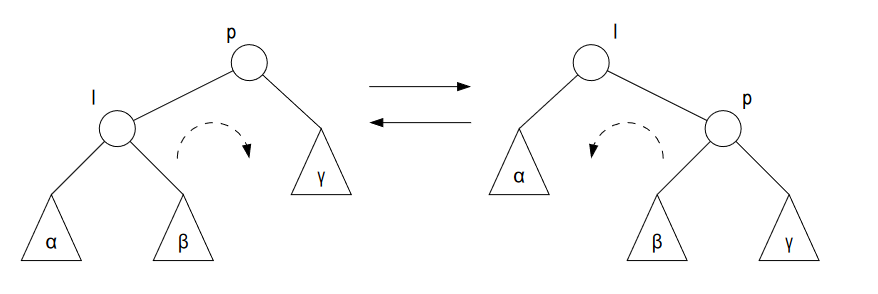
\includegraphics[width=0.5\textwidth]{rotations}
    \caption{Rotaties.}
    \label{fig:rotations}
\end{figure}
\begin{itemize}
    \item Een rotatie (figuur \ref{fig:rotations}) wijzigt de vorm van de boom, maar behoudt de inorder volgorde van de sleutels.
    \item Er moeten enkel pointers aangepast worden, en is dus $O(1)$.
\end{itemize}

\subsection{Bottom-up rood-zwarte bomen}
\subsubsection{Toevoegen}
\begin{itemize}
    \item De knoop wordt eerst op de gewone manier toegevoegd.
    \item Welke kleur geven we die knoop?
    \begin{itemize}
        \item \textbf{Zwart:} dit kan de zwarte hoogte van veel knopen ontregelen.
        \item \textbf{Rood:} dit mag enkel als de ouder zwart is.
        \item Kies voor rood omdat zwarte hoogte moeilijker te herstellen valt.
    \end{itemize}
    \item Enkel een probleem als de ouder rood is: deze storing wordt verwijderd door rotaties en kleurwijzigingen door te voeren.
    \item Vaststellingen:
    \begin{itemize}
        \item De ouder $p$ van de nieuwe knoop $c$ is rood.
        \item De grootouder $g$ van $c$ is zwart want $p$ is rood.
    \end{itemize}
    \item Er zijn zes mogelijke gevallen, die twee groepen van drie vormen, naar gelang dat $p$ een linker- of rechterkind is van $g$. 
    \item We onderstellen dat $p$ een linkerkind is van $g$. 
    \begin{enumerate}
        \item \textbf{De broer $b$ van $p$ is rood.}
        \begin{figure}[ht]
            \centering
            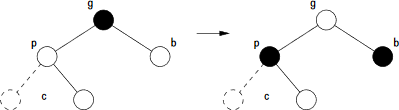
\includegraphics[width=0.5\textwidth]{rbt_bottomup_case1}
            \caption{$b$ is rood; de ligging van $c$ is onbelangrijk.}
            \label{fig:rbt_bottomup_case1}
        \end{figure}
        \begin{itemize}
            \item Het probleem wordt opgeschoven in de richting van de wortel.
        \end{itemize}
        \item \textbf{De broer $b$ van $p$ is zwart.}
        \begin{enumerate}
            \item \textbf{Knoop $c$ is een linkerkind van $p$.}
            \begin{figure}[ht]
                \centering
                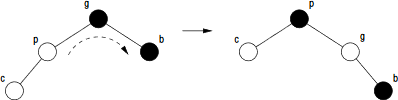
\includegraphics[width=0.5\textwidth]{rbt_bottomup_case2}
                \caption{$b$ is zwart en $c$ ligt aan de buitenkant.}
                \label{fig:rbt_bottomup_case2}
            \end{figure}
            \item \textbf{Knoop $c$ is een rechterkind van $p$.}
            \begin{figure}[ht]
                \centering
                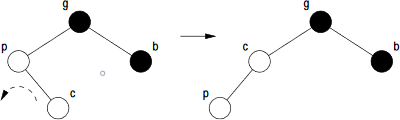
\includegraphics[width=0.5\textwidth]{rbt_bottomup_case3}
                \caption{$b$ is zwart en $c$ ligt aan de binnenkant.}
                \label{fig:rbt_bottomup_case3}
            \end{figure}
        \end{enumerate}
    \end{enumerate}
    \item Hoogstens 2 rotaties om de boom te herstellen, voorafgegaan door eventueel $O(\lg n)$ opschuivingen.
    \item Roteren en opschuiven is $O(1)$, en afdalen is $O(\lg n)$ zodat toevoegen $O(\lg n)$ is.
\end{itemize}


\subsubsection{Verwijderen}
\begin{itemize}
    \item Verwijderen in een normale zoekboom kent drie gevallen:
    \begin{enumerate}
        \item De te verwijderen knoop heeft geen kinderen.
        \item De te verwijderen knoop heeft één kind.
        \item De te verwijderen knoop heeft twee kinderen. 
        \begin{itemize}
            \item Dit geval wordt omgevormd naar één van de twee vorige gevallen door de voorloper of opvolger te zoeken (die ofwel geen kinderen of één kind hebben) en de sleutels om te wisselen. De te verwijderen knoop wordt dan de fysische locatie van de voorloper of opvolger. 
        \end{itemize}
    \end{enumerate}

    \item Deze laatste stap kan nu twee vormen aannemen:
    \begin{enumerate}
        \item Als de te verwijderen knoop rood is, is er geen gevolg voor de zwarte hoogte en is de operatie klaar.
        \item Als de te verwijderen knoop zwart is, zijn er twee mogelijkheden:
        \begin{enumerate}
            \item \textbf{De knoop heeft één rood kind.} Dit rood kind kan de zwarte kleur overnemen, zodat de zwarte hoogten intact blijven.
            \item \textbf{De knoop heeft twee virtuele zwarte kinderen.} De zwarte kleur wordt aan één van de kinderen gegeven, zodat die \textbf{dubbelzwart} wordt.
        \end{enumerate}
    \end{enumerate}

    \item In het eerste geval is de operatie klaar. In het tweede geval moet de boom, die nu een dubbelzwarte knoop bevat, herstelt worden.
    \item Als de dubbelzwarte knoop $c$ de wortel is, kan deze extra zwarte kleur verdwijnen. 
    \item Als $c$ geen wortel is, en ouder $p$ heeft, dan zijn er acht mogelijkheden die in groepen van twee uiteenvallen naargelang $c$ een linker- of rechterkind van $p$ is.
    \item We veronderstellen dat $c$ een linkerkind is van $p$.
    \begin{enumerate}
        \item \textbf{De broer $b$ van $c$ is zwart.} De kleur van $p$ is willekeurig. Hier zijn er drie gevallen mogelijk, afhankelijk van de kleur van de kinderen van $b$.
        \begin{enumerate}
            \item \textbf{Broer $b$ heeft twee zwarte kinderen}.
            \begin{figure}[ht]
                \centering
                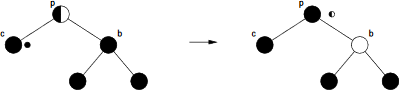
\includegraphics[width=0.5\textwidth]{rbt_bottomup_case4}
                \caption{Zwarte broer, zwarte neven.}
                \label{fig:rbt_bottomup_case4}
            \end{figure}
            \begin{itemize}

                \item Als $p$ rood was, dan is de operatie gelukt.
                \item Als $p$ reeds zwart was, dan verschuift het probleem zich naar boven.
            \end{itemize}
            \item \textbf{Broer $b$ heeft een rood rechterkind}. De kleur van het linkerkind $l$ van $b$ is willekeurig.
            \begin{figure}[ht]
                \centering
                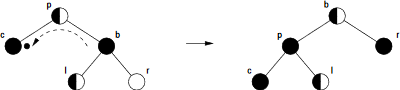
\includegraphics[width=0.5\textwidth]{rbt_bottomup_case5}
                \caption{Rode neef langs buiten.}
                \label{fig:rbt_bottomup_case5}
            \end{figure}
            \item \textbf{Broer $b$ heeft een zwarte rechterkind en een rood linkerkind}.
            \begin{figure}[ht]
                \centering
                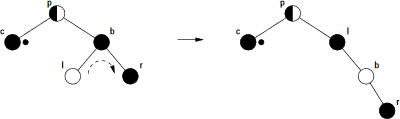
\includegraphics[width=0.5\textwidth]{rbt_bottomup_case6}
                \caption{Rode neef langs buiten.}
                \label{fig:rbt_bottomup_case6}
            \end{figure}
            \begin{itemize}
                \item Dit is nu het vorige geval.
            \end{itemize}
        \end{enumerate}
        \item \textbf{De broer $b$ van $c$ is rood}.
        \begin{figure}[ht]
            \centering
            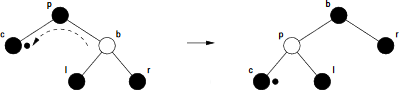
\includegraphics[width=0.5\textwidth]{rbt_bottomup_case7}
            \caption{Rode broer.}
            \label{fig:rbt_bottomup_case7}
        \end{figure}
        \begin{itemize}
            \item Dit is nu het eerste geval.
        \end{itemize}
    \end{enumerate}
    \item Hoogstens 3 rotaties nodig om de boom te herstellen, voorafgegaan door eventueel $O(\lg n)$ opschuivingen.
    \item Roteren en opschuiven is $O(1)$, en afdalen is $O(\lg n)$ zodat verwijderen $O(\lg n)$ is.
\end{itemize}


\subsection{Top-down rood-zwarte bomen}
\subsubsection{Toevoegen}
\begin{itemize}
    \item Ook hier worden nieuwe knopen rood gemaakt.
    \item Op de weg naar beneden mogen er geen rode broers zijn.
    \item Als we een \textbf{zwarte knoop met twee rode kinderen} tegenkomen, dan maken we die knoop rood en zijn kinderen zwart.
    \item Als zijn ouder rood is, kan dit met rotaties en kleurwijzigingen opgelost worden.
    \item Toevoegen daalt enkel in de boom en is $O(\lg n)$.
\end{itemize}

\subsubsection{Verwijderen}
\begin{itemize}
    \item De zwarte hoogte van de fysisch te verwijderen knoop is één, omdat minstens één van zijn kinderen virtueel is.
    \item Om geen problemen te krijgen met de zwarte hoogte moet deze knoop rood zijn, maar dan moet zijn tweede kind ook virtueel zijn.
    \item De zoekknoop kan eender waar in de boom zitten, daarom wordt elke bolgende knoop op de zoekweg rood gemaakt.
    \begin{itemize}
        \item Tijdens het afdalen komen we in een rode of rood gemaakte knoop $p$.
        \item Die heeft dan zeker een zwart kind $c$, dat rood moet worden.
        \item Er zijn acht mogelijkheden die in groepen van twee uiteenvallen naargelang $c$ een linker- of rechterkind van $p$ is.
    \end{itemize}
    \item We veronderstellen dat $c$ een linkerkind is van $p$.
    \begin{enumerate}
        \item \textbf{Knoop $c$ heeft minstens één rood kind.}
        \begin{figure}[ht]
            \centering
            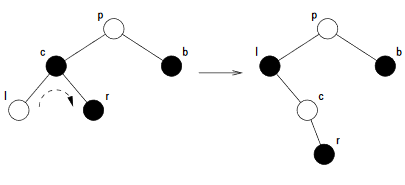
\includegraphics[width=0.5\textwidth]{rbt_topdown_case1}
            \caption{}
            \label{fig:rbt_topdown_case1}
        \end{figure}
        \begin{itemize}
            \item Als we naar een rode knoop moeten afdalen zitten we terug in de beginsituatie.
            \item Als $c$ de fysisch te verwijderen knoop is of als we naar een zwarte knoop moeten afdalen:
            \begin{itemize}
                \item Roteer $c$ samen met zijn rood kind zodat $c$ nu als ouder zijn oorspronkelijk rood kind heeft.
                \item Wijzig de kleur van $c$ naar zwart.
                \item Wijzig de kleur van zijn oorspronkelijk kind naar rood.
            \end{itemize}
        \end{itemize}
        \item \textbf{Knoop $c$ heeft twee zwarte kinderen.}
        \begin{figure}[ht]
            \centering
            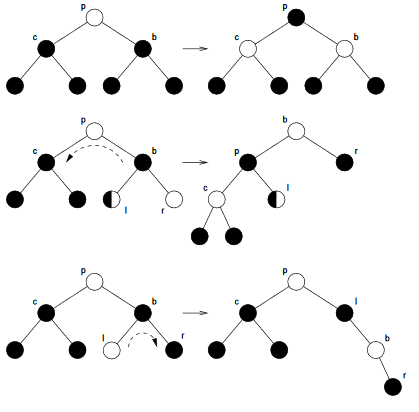
\includegraphics[width=0.5\textwidth]{rbt_topdown_case2}
            \caption{}
            \label{fig:rbt_topdown_case2}
        \end{figure}
        
    \end{enumerate}

\end{itemize}


%\subsection{Vereenvoudigde rood-zwarte bomen}
%\begin{itemize}
%    \item De implementatie is omslachtig door de talrijke speciale gevallen.
%    \item Eenvoudigere varianten bestaan:
%    \begin{itemize}
%        \item Een \textbf{AA-boom} geeft aan dat enkel een rechterkind rood moet zijn.
%        \item Een \textbf{Binary B-tree} beperkt het aantal gevallen maar behouden toch de asymptotische efficiëntie.
%        \item Een \textbf{left-leaning red-black-tree} stelt de eis dat een zwarte knoop enkel een rood rechterkind mag hebben als het reeds een rood linkerkind heeft.
%    \end{itemize}
%\end{itemize}
\section{Splaybomen}
\label{sec:splaybomen}
\begin{itemize}
    \item Garanderen dat elke reeks opeenvolgende operaties efficiënt is.
    \item Als we $m$ operaties verrichten op de splay tree, waarbij $n$ keer toevoegen, dan is de performantie van deze reeks $O(m \lg n)$. 
    \item Uitgemiddeld is dit $O(\lg n)$.
    \item Individuelde operaties mogen inefficiënt zijn, maar de boom moet zo aangepast worden zodat een reeks van die operaties efficiënt zijn.
    \item \textbf{Basisidee:} Elke knoop die gezocht wordt, toegevoegd of verwijdert wordt, zal de wortel worden van de boom, zodat opeenvolgende operaties op die knoop efficiënt zijn.
    \item Een willekeurige knoop tot wortel maken gebeurd via de \textbf{\textit{splay-operatie}}.
    \item De weg naar een diepe knoop bevat knopen die ook diep liggen. Terwijl we een knoop wortel maken, moeten de knopen op het zoekpad ook aangepast worden, zodat ook de toegangstijd van deze knopen verbetert, anders blijft de kans bestaan dat een reeks van operaties inefficiënt is.
    \item Er moet geen extra informatie bijgehouden worden voor knopen, wat geheugen uitspaart. 
    \item De splay-operatie is gedefinieerd voor zowel bottom-up als top-down splaybomen.
\end{itemize}

\subsection{Bottom-up splayboom}
\begin{figure}[ht]
    \centering
    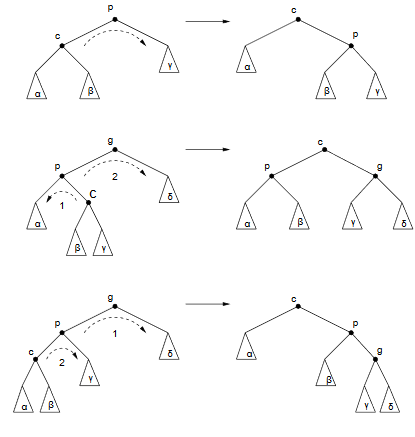
\includegraphics[width=0.5\textwidth]{splay_bottomup}
    \caption{Bottom-up splay.}
    \label{fig:splay_bottomup}
\end{figure}
\begin{itemize}
    \item De knoop wordt eerst gezocht zoals bij een gewone zoekboom.
    \item De splay-operatie gebeurt van onder naar boven.
    \item Een knoop kan naar boven gebracht worden door hem telkens te roteren met zijn ouder.
    \item Om de toegangstijd van knopen op de zoekweg ook te verbeteren, zijn er drie verschillende mogelijkheden:
    \begin{enumerate}
        \item \textbf{De ouder $p$ van $c$ is wortel}. 
        \begin{itemize}
            \item Standaard rotatie.
        \end{itemize}
        \item \textbf{Knoop $c$ heeft nog een grootouder}.
        \begin{itemize}
            \item Er zijn vier gevallen, die uitvallen in groepen van twee, naar gelang dat $p$ een linker- of rechterkind is van grootouder $g$.
            \item We veronderstellen dat $p$ linkerkind is van $g$.
        \end{itemize}
        
        \begin{enumerate}
            \item \textbf{Knoop $c$ is een rechterkind van $p$}.
            \begin{itemize}
                \item Roteer $p$ en $c$ naar links.
                \item Roteer $g$ en $c$ naar rechts.
            \end{itemize}
            \item \textbf{Knoop $c$ is een linkerkind van $p$}.
            \begin{itemize}
                \item Roteer $g$ en $p$ naar rechts.
                \item Roteer $p$ en $c$ naar rechts.
            \end{itemize}
        \end{enumerate}
    \end{enumerate}
    \item De \textbf{woordenboekoperaties verlopen nu als volgt:}
    \begin{itemize}
        \item \textbf{Zoeken.} De knoop wordt eerst gezocht zoals een gewone zoekboom. Daarna wordt deze tot wortel gemaakt via de splay-operatie. 
        \item \textbf{Toevoegen.} Toevoegen gebeurt ook zoals een gewone zoekboom. De nieuwe knoop wordt dan tot wortel gemaakt met de splay-operatie.
        \item \textbf{Verwijderen.} Verwijderen gebeurt ook zoals een gewone zoekboom. Daarna wordt de ouder van die knoop tot wortel gemaakt met de splay-operatie.
    \end{itemize}
\end{itemize}
\subsection{Top-down splayboom}
\begin{figure}[ht]
    \centering
    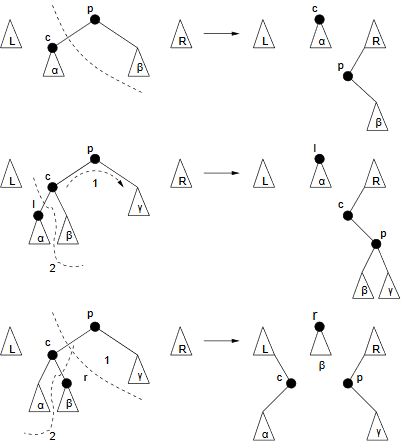
\includegraphics[width=0.5\textwidth]{splay_topdown}
    \caption{Top-down splay.}
    \label{fig:splay_topdown}

\end{figure}
\begin{itemize}
    \item De splayoperatie wordt uitgevoerd tijdens de afdaling, zodat de gezochte knoop wortel zal zijn als we hem bereiken.
    \item De boom wordt in drie zoekbomen opgedeeld, $L$, $M$ en $R$.
    \begin{itemize}
        \item Alle sleutels in $L$ zijn kleiner dan die in $M$.
        \item Alle sleutels in $R$ zijn groter dan die in $M$.
    \end{itemize}
    \item Eerst is $M$ de oorspronkelijke boom en zijn $L$ en $R$ ledig.
    \item De huidige knoop op de zoekweg is steeds de wortel van $M$.
    \item Stel dat we bij een knoop $p$ uitkomen, en dan nog verder moeten naar een knoop $c$.
    \item Er zijn dan twee groepen van 3 gevallen, afhankelijk of $c$ een linker- of rechterkind is van $p$.
    \item We veronderstellen dat $c$ een linkerkind is van $p$.
    \begin{enumerate}
        \item \textbf{Knoop $c$ is de laatste knoop op de zoekweg.}
        \begin{itemize}
            \item Knoop $p$ wordt het nieuwe kleinste element in $R$ samen met zijn rechtse deelboom.
            \item Knoop $c$ wordt de wortel van $M$.
        \end{itemize}
        \item \textbf{Knoop $c$ is niet de laatste knoop op de zoekweg.}
        \begin{itemize}
            \item \textbf{We moeten verder afdalen naar het linkerkind $l$ van $c$.}
            \begin{itemize}
                \item Roteer $p$ en $c$ naar rechts.
                \item Knoop $c$ wordt het kleinste element in $R$ samen met de rechtse deelboom van $c$.
                \item De linkse deelboom van $c$ wordt de nieuwe $M$ met als wortel $l$.
            \end{itemize}
            \item \textbf{We moeten verder afdalen naar het rechterkind $r$ van $c$.}
            \begin{itemize}
                \item Knoop $p$ wordt het kleinste element in $R$ samen met de rechtse deelboom van $p$.
                \item Knoop $c$ wordt het nieuwe grootste element in $L$.
                \item De rechtse deelboom van $c$ wordt de nieuwe $M$ met als wortel $r$.
            \end{itemize}
        \end{itemize}
    \end{enumerate}
    \item Als de gezochte knoop $c$ wortel van $M$ is, wordt de splayoperatie afgerond met een \textbf{join-operatie}.
    \begin{figure}[ht]
        \centering
        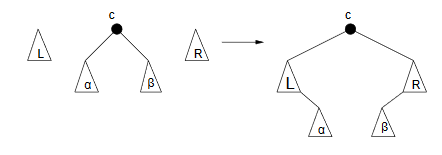
\includegraphics[width=0.5\textwidth]{splay_join}
        \caption{Samenvoegen na top-down splayen.}
        \label{fig:splay_join}
    \end{figure}
    \item De \textbf{woordenboekoperaties verlopen nu als volgt:}
    \begin{itemize}
        \item \textbf{Zoeken.} De knoop met de gezochte sleutel wordt tot wortel gemaakt. Als de sleutel niet gevonden wordt dan is zijn opvolger of voorloper de wortel.
        \item \textbf{Toevoegen.} Analoog aan de alternatieve versie bottom-up.
        \item \textbf{Verwijderen.} Analoog aan de alternatieve versie bottom-up.
    \end{itemize}
\end{itemize}

\subsection{Performantie van splay trees}
\begin{itemize}
    \item Niet eenvoudig aangezien vorm van de boom vaak verandert.
    \item We willen aantonen dat een reeks van $m$ operaties op een splay tree met maximaal $n$ knopen een performantie van $O(m\lg n)$ heeft.
    \item Er wordt een \textbf{potentiaalfunctie} $\Phi$ gebruikt.
    \item Elke mogelijke vorm van een splayboom krijgt een reeël getal toegewezen aan de hand van deze potentiaalfunctie.
    \item Efficiënte operaties die minder tijd gebruiken dan de geamortiseerde tijd per operatie doen het potentiaal stijgen.
    \item Niet-efficiënte operaties die meer tijd gebruiken dan de geamortiseerde tijd per operatie doen het potentiaal dalen.
    \item De geamortiseerde tijd van een operatie wordt gedefinieerd als de som van haar werkelijke tijd en de toename van het potentiaal.
    \begin{itemize}
        \item Stel $t_i$ de werkelijke tijd van de $i-$de operatie.
        \item Stel $a_i$ de geamortiseerde tijd van die operatie.
        \item Stel $\Phi_i$ het potentiaal na deze operatie.
        $$\rightarrow a_i = t_i + \Phi_{i} - \Phi_{i - 1}$$
    \end{itemize}
    \item De geamortiseerde tijd van een reeks $m$ operaties is de som van de individuelde geamortiseerde tijden:
    \begin{equation*}
        \begin{split}
            \sum_{i=1}^m a_i &= \sum_{i=1}^m (t_i + \Phi_{i} - \Phi_{i - 1}) \\
                             &= t_1 + \Phi_1 - \Phi_0 + t_2 + \Phi_2 - \Phi_1 + t_3 + \Phi_3 - \Phi_2 + \dots + t_m + \Phi_m - \Phi_{m - 1} \\
                             &= \Phi_{m} - \Phi_{0} + \sum_{i=1}^m t_i
        \end{split}
    \end{equation*}
    \item Als de potentiaalfunctie zo gekozen wordt zodat het eindpotentiaal $\Phi_m$ zeker niet kleiner is dan de beginpotentiaal $\Phi_0$, dan vormt de totale geamortiseerde tijd een \textbf{bovengrens} van de werkelijke tijd want de boom zal zeker niet slechter zijn.
    \item De eenvoudigste potentiaalfunctie geeft voor elke knoop $i$ een gewicht $s_i$ die gelijk is aan het aantal knopen in de deelboom waarvan hij wortel is. De potentiaal van de boom is dan de som van de logaritmen van deze gewichten:
    $$\Phi = \sum_{i=1}^n \lg s_i$$
    \item We noemen $\lg s_i$ de rang $r_i$ van knoop $i$.
    \item Performantie-analyse van bottom-up splayboom:
    \begin{itemize}
        \item Performantie is evenredig met de diepte van de knoop, en dus met het aantal uitgevoerde rotaties.
        \item We willen aantonen dat de geamortiseerde tijd voor het zoeken naar een knoop $c$ gevolgd door een splay-operatie op die knoop gelijk is aan $$O(1 + 3(r_w - r_c))$$
        waarbij $r_w$ de rang van de wortel is en $r_c$ de rang van de gezochte knoop.
        \begin{itemize}
            \item Als $c$ reeds de wortel is, dan is $r_w = r_c$ en blijft het potentiaal dezelfde.
            $$O(1 + 3(r_w - r_c)) = O(1)$$
            \item Anders moeten zoveel splay-operaties uitgevoerd worden als de diepte van de knoop (moet niet gekend zijn).
            \begin{itemize}
                \item Een zig wijzigt de rang van $c$ en $p$
                $$a < 1 + r'_c - r_c$$

                \item Een zig-zag wijzigt de rang van $c$, $p$ en $g$
                $$a < 2(r'_c - r_c)$$

                \item Een zig-zig wijzigt de rang van $c$, $p$ en $g$
                $$a <3(r'_c - r_c)$$ 
            \end{itemize}
        \end{itemize}
        \item De bovengrenzen voor de drie operaties bevatten dezelfde positieve term $r'_c - r_c$ maar met verschillende coëfficiënten.
        \item De totale geamortiseerde tijd is een som van dergerlijke bovengrenzen, maar kan niet vereenvoudigt worden als coëfficiënten niet gelijk zijn.
        \item Aangezien het bovengrenzen zijn, wordt de grootste coëfficiënt genomen.
        \item In de som vallen de meeste termen nu weg, behalve de rang van $c$ voor en na de volledige splay-operatie.
        \item De geamortiseerde tijden van de woordenboekoperaties op een bottom-splay tree met $n$ knopen zijn nu:
        \begin{itemize}
            \item \textbf{Zoeken.} $O(1 + 3\lg n)$ want $s_w = n$.
            \item \textbf{Toevoegen.} $O(1 + 4\lg n)$.

            Op de zoekweg worden de rang van knopen $p_1,p_2, ... p_k$ op de zoekweg gewijzigt. Stel $s_{p_{i}}$ het gewicht van knoop $p_i$ voor het toevoegen en $s'_{p_{i}}$ het gewicht van knoop $p_i$ na het toevoegen. Gebruik makend van de regel $\lg(s'_{p_{i}}) - \lg(s_{p_{i}}) = \lg\frac{s'_{p_{i}}}{s_{p_{i}}}$ wordt de potentiaaltoename gedefinieerd als
            $$\lg\bigg(\frac{s'_{p_{1}}}{s_{p_{1}}}\bigg) + \lg\bigg(\frac{s'_{p_{2}}}{s_{p_{2}}}\bigg) + \cdots + \lg\bigg(\frac{s'_{p_{k}}}{s_{p_{k}}}\bigg) = \lg\bigg(\frac{s'_{p_{1}}}{s_{p_{1}}}\frac{s'_{p_{2}}}{s_{p_{2}}}\cdots\frac{s'_{p_{k}}}{s_{p_{k}}}\bigg)$$
            Deze is nooit groter dan $$\lg\bigg(\frac{s'_{p_{1}}}{s_{p_{k}}}\bigg) \leq \lg(n + 1)$$
            \item \textbf{Verwijderen.} Het effect van verwijderen is nooit positief.
        \end{itemize}
        \item De geamortiseerde tijd voor een reeks van $m$ woordenboekoperaties is de som van de geamortiseerde tijden voor de individuele operaties.
        \item Stel $n_i$ het aantal knopen bij de $i-$de operatie dan wordt die tijd $O(m + 4\sum_{i=1}^m\lg n_i) = O(m + 4m\lg n) = O(m\lg n)$.
    \end{itemize}
\end{itemize}

\section{Gerandomiseerde zoekbomen}
\label{sec:gerandomiseerde-zoekbomen}
\begin{itemize}
    \item De performantie van de woordenboekoperaties op een gewone zoekboom is $O(\lg n)$ als elke toevoegvolgorde even waarschijnlijk is.
    \item Gerandomiseerde zoekbomen maken gebruik van een random generator om de operatievolgorde te neutraliseren.
    \item Deze bomen blijven steeds random.
    \item Een \textbf{treap} is een gerandomiseerde zoekboom.
    \begin{itemize}
        \item Elke knoop krijgt naast een sleutel ook een prioriteit, die door de random generator wordt toegekend als de knoop toegevoegd wordt.
        \item De prioriteiten van de knopen voldoen aan de heapvoorwaarde: de prioriteit van een kind is maximaal even hoog als die van zijn ouder.
    \end{itemize}
    \item De woordenboekoperaties:
    \begin{itemize}
        \item \textbf{Zoeken.}  Zoeken moet geen rekening houden met de prioriteiten en verloopt zoals een normale binaire zoekboom.
        \item \textbf{Toevoegen.} Eerst wordt er normaal toegevoegd. De knoop wordt nadien naar boven geroteerd om aan de heapvoorwaarde te voldoen.
        \item \textbf{Verwijderen.} De te verwijderen knoop krijgt de laagste prioriteit, zodat die naar beneden geroteerd wordt. Dit blad kan dan verwijdert worden.
    \end{itemize}
\end{itemize}

\section{Skip lists}
\begin{figure}[ht]
    \centering
    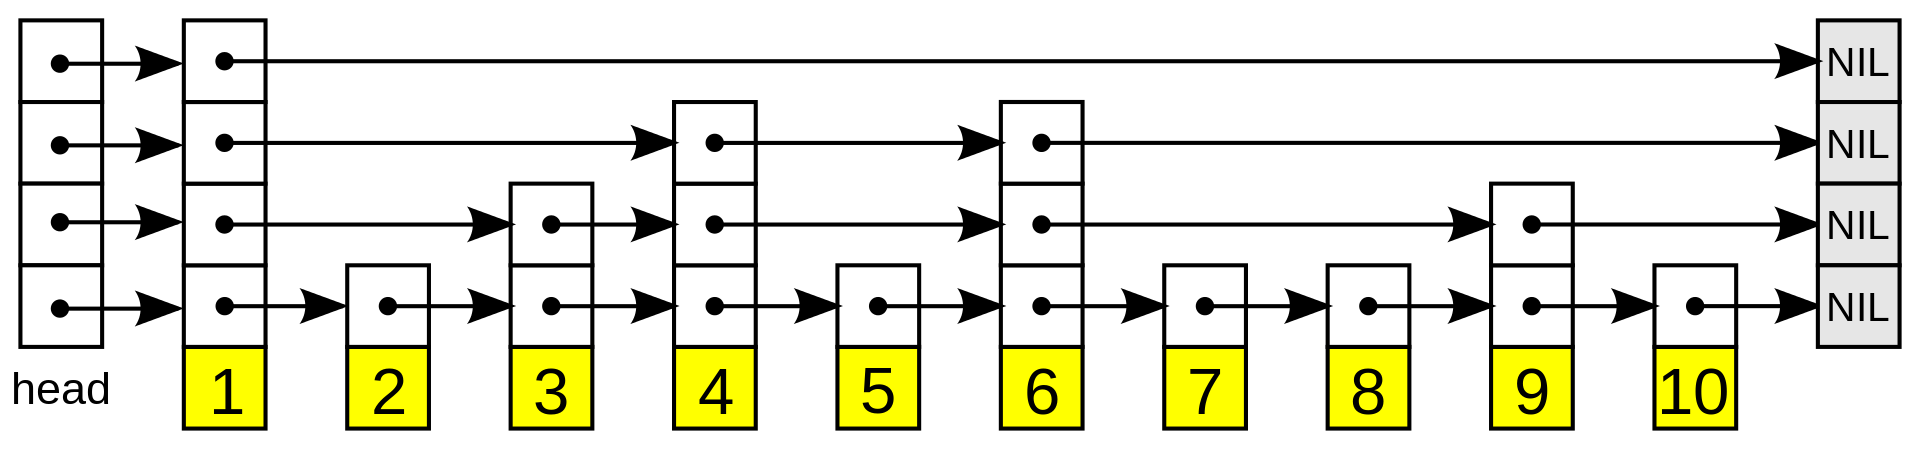
\includegraphics[width=\textwidth]{skip_list}
    \caption{Een skip list.}
    \label{fig:skip_list}
\end{figure}
\begin{itemize}
    \item Een meerwegszoekboom geïmplementeerd met gelinkte lijsten.
    \item Alle bladeren zitten op dezelfde diepte.
    \item Elke lijstknoop heeft plaats voor één sleutel en één kindwijzer.
    \item Een knoop met $k$ kinderen bevat $k-1$ sleutels, zodat er één sleutelplaats over blijft.
\end{itemize}